% Created by tikzDevice version 0.6.2-92-0ad2792 on 2013-02-01 15:13:44
% !TEX encoding = UTF-8 Unicode
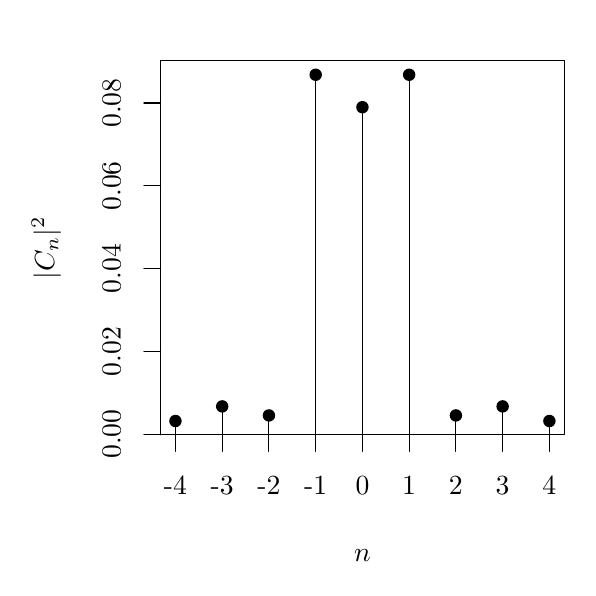
\begin{tikzpicture}[x=1pt,y=1pt]
\definecolor[named]{fillColor}{rgb}{1.00,1.00,1.00}
\path[use as bounding box,fill=fillColor,fill opacity=0.00] (0,0) rectangle (195.13,195.13);
\begin{scope}
\path[clip] ( 48.00, 48.00) rectangle (193.93,183.13);
\definecolor[named]{fillColor}{rgb}{0.00,0.00,0.00}

\path[fill=fillColor] (104.07,178.12) circle (  2.25);

\path[fill=fillColor] ( 87.18, 55.01) circle (  2.25);

\path[fill=fillColor] ( 70.29, 58.28) circle (  2.25);

\path[fill=fillColor] ( 53.40, 53.00) circle (  2.25);

\path[fill=fillColor] (137.85,178.12) circle (  2.25);

\path[fill=fillColor] (154.74, 55.01) circle (  2.25);

\path[fill=fillColor] (171.63, 58.28) circle (  2.25);

\path[fill=fillColor] (188.52, 53.00) circle (  2.25);
\end{scope}
\begin{scope}
\path[clip] (  0.00,  0.00) rectangle (195.13,195.13);
\definecolor[named]{drawColor}{rgb}{0.00,0.00,0.00}

\path[draw=drawColor,line width= 0.4pt,line join=round,line cap=round] ( 48.00, 48.22) -- ( 48.00,167.89);

\path[draw=drawColor,line width= 0.4pt,line join=round,line cap=round] ( 48.00, 48.22) -- ( 42.00, 48.22);

\path[draw=drawColor,line width= 0.4pt,line join=round,line cap=round] ( 48.00, 78.14) -- ( 42.00, 78.14);

\path[draw=drawColor,line width= 0.4pt,line join=round,line cap=round] ( 48.00,108.05) -- ( 42.00,108.05);

\path[draw=drawColor,line width= 0.4pt,line join=round,line cap=round] ( 48.00,137.97) -- ( 42.00,137.97);

\path[draw=drawColor,line width= 0.4pt,line join=round,line cap=round] ( 48.00,167.89) -- ( 42.00,167.89);

\node[text=drawColor,rotate= 90.00,anchor=base,inner sep=0pt, outer sep=0pt, scale=  1.00] at ( 33.60, 48.22) {0.00};

\node[text=drawColor,rotate= 90.00,anchor=base,inner sep=0pt, outer sep=0pt, scale=  1.00] at ( 33.60, 78.14) {0.02};

\node[text=drawColor,rotate= 90.00,anchor=base,inner sep=0pt, outer sep=0pt, scale=  1.00] at ( 33.60,108.05) {0.04};

\node[text=drawColor,rotate= 90.00,anchor=base,inner sep=0pt, outer sep=0pt, scale=  1.00] at ( 33.60,137.97) {0.06};

\node[text=drawColor,rotate= 90.00,anchor=base,inner sep=0pt, outer sep=0pt, scale=  1.00] at ( 33.60,167.89) {0.08};

\path[draw=drawColor,line width= 0.4pt,line join=round,line cap=round] ( 48.00, 48.00) --
	(193.93, 48.00) --
	(193.93,183.13) --
	( 48.00,183.13) --
	( 48.00, 48.00);
\end{scope}
\begin{scope}
\path[clip] (  0.00,  0.00) rectangle (195.13,195.13);
\definecolor[named]{drawColor}{rgb}{0.00,0.00,0.00}

\node[text=drawColor,anchor=base,inner sep=0pt, outer sep=0pt, scale=  1.00] at (120.96,  2.40) {$n$};

\node[text=drawColor,rotate= 90.00,anchor=base,inner sep=0pt, outer sep=0pt, scale=  1.00] at (  9.60,115.56) {$|C_n|^2$};
\end{scope}
\begin{scope}
\path[clip] ( 48.00, 48.00) rectangle (193.93,183.13);
\definecolor[named]{drawColor}{rgb}{0.00,0.00,0.00}

\path[draw=drawColor,line width= 0.4pt,line join=round,line cap=round] (137.85, 48.22) --
	(137.85,178.12);

\path[draw=drawColor,line width= 0.4pt,line join=round,line cap=round] (154.74, 48.22) --
	(154.74, 55.01);

\path[draw=drawColor,line width= 0.4pt,line join=round,line cap=round] (171.63, 48.22) --
	(171.63, 58.28);

\path[draw=drawColor,line width= 0.4pt,line join=round,line cap=round] (188.52, 48.22) --
	(188.52, 53.00);

\path[draw=drawColor,line width= 0.4pt,line join=round,line cap=round] (104.07, 48.22) --
	(104.07,178.12);

\path[draw=drawColor,line width= 0.4pt,line join=round,line cap=round] ( 87.18, 48.22) --
	( 87.18, 55.01);

\path[draw=drawColor,line width= 0.4pt,line join=round,line cap=round] ( 70.29, 48.22) --
	( 70.29, 58.28);

\path[draw=drawColor,line width= 0.4pt,line join=round,line cap=round] ( 53.40, 48.22) --
	( 53.40, 53.00);
\definecolor[named]{fillColor}{rgb}{0.00,0.00,0.00}

\path[fill=fillColor] (120.96,166.39) circle (  2.25);

\path[draw=drawColor,line width= 0.4pt,line join=round,line cap=round] (120.96, 48.22) --
	(120.96,166.39);
\end{scope}
\begin{scope}
\path[clip] (  0.00,  0.00) rectangle (195.13,195.13);
\definecolor[named]{drawColor}{rgb}{0.00,0.00,0.00}

\path[draw=drawColor,line width= 0.4pt,line join=round,line cap=round] ( 53.40, 48.00) -- (188.52, 48.00);

\path[draw=drawColor,line width= 0.4pt,line join=round,line cap=round] ( 53.40, 48.00) -- ( 53.40, 42.00);

\path[draw=drawColor,line width= 0.4pt,line join=round,line cap=round] ( 70.29, 48.00) -- ( 70.29, 42.00);

\path[draw=drawColor,line width= 0.4pt,line join=round,line cap=round] ( 87.18, 48.00) -- ( 87.18, 42.00);

\path[draw=drawColor,line width= 0.4pt,line join=round,line cap=round] (104.07, 48.00) -- (104.07, 42.00);

\path[draw=drawColor,line width= 0.4pt,line join=round,line cap=round] (120.96, 48.00) -- (120.96, 42.00);

\path[draw=drawColor,line width= 0.4pt,line join=round,line cap=round] (137.85, 48.00) -- (137.85, 42.00);

\path[draw=drawColor,line width= 0.4pt,line join=round,line cap=round] (154.74, 48.00) -- (154.74, 42.00);

\path[draw=drawColor,line width= 0.4pt,line join=round,line cap=round] (171.63, 48.00) -- (171.63, 42.00);

\path[draw=drawColor,line width= 0.4pt,line join=round,line cap=round] (188.52, 48.00) -- (188.52, 42.00);

\node[text=drawColor,anchor=base,inner sep=0pt, outer sep=0pt, scale=  1.00] at ( 53.40, 26.40) {-4};

\node[text=drawColor,anchor=base,inner sep=0pt, outer sep=0pt, scale=  1.00] at ( 70.29, 26.40) {-3};

\node[text=drawColor,anchor=base,inner sep=0pt, outer sep=0pt, scale=  1.00] at ( 87.18, 26.40) {-2};

\node[text=drawColor,anchor=base,inner sep=0pt, outer sep=0pt, scale=  1.00] at (104.07, 26.40) {-1};

\node[text=drawColor,anchor=base,inner sep=0pt, outer sep=0pt, scale=  1.00] at (120.96, 26.40) {0};

\node[text=drawColor,anchor=base,inner sep=0pt, outer sep=0pt, scale=  1.00] at (137.85, 26.40) {1};

\node[text=drawColor,anchor=base,inner sep=0pt, outer sep=0pt, scale=  1.00] at (154.74, 26.40) {2};

\node[text=drawColor,anchor=base,inner sep=0pt, outer sep=0pt, scale=  1.00] at (171.63, 26.40) {3};

\node[text=drawColor,anchor=base,inner sep=0pt, outer sep=0pt, scale=  1.00] at (188.52, 26.40) {4};
\end{scope}
\end{tikzpicture}
